\documentclass{ctexart}
\usepackage{graphicx}
\usepackage{ctex}
\usepackage{listings}

\usepackage{tikz}
\usetikzlibrary{arrows, decorations.pathmorphing, backgrounds, positioning, fit, petri, automata}
\definecolor{yellow1}{rgb}{1,0.8,0.2}




\author{xzx}
\title{assignment2我的答案}


\begin{document}
\maketitle
\setcounter{page}{0}
\thispagestyle{empty}
\newpage

\begin{flushleft}

\section{Q1: Fully-connected Neural Network}

\subsection{/cs231n/layers.py}

\subsubsection{affine\_forward \& affine\_backward}
\paragraph{affine\_forward}没什么好说的,就是正常的相乘就完了。\\
\paragraph{affine\_backward}需要注意的地方是再对dout求和的时候,参数keepdims=True很有用。假设
dout是(N,M)的矩阵,
\begin{lstlisting}[language=python]
  np.sum(dout,axis=0)#返回一个(M,)的矩阵
  np.sum(dout,axis=0,keepdims=True)#返回一个(1,M)的矩阵
\end{lstlisting}


\subsubsection{/cs231n/classifiers/fc\_net/py}
\paragraph{TwoLayerNet}
与assignment1不同的是,这里的两层网络加上了一个relu层。在做作业的时候,开始忘掉了relu层,
导致不论怎么调hyper parameter训练集上面的accuracy最高只能到达43\%。因为affine层是线性
层,线性层不论怎么叠加的效果都是线性层,所以没有relu的情况下准确率很难提高

\subsection{update rules}
课程中介绍了几种主流的更新W的方法。想象当前所在的位置是山谷中随机的一个位置,目标是走到山谷
的底部。\\
最简单的就是SGD,每次按照偏导数的方向(下山的方向)走一小步,直到走到结束条件为止。\\
第二种方法是Momentum。假如一个小球从山谷的某个地方向下滚,这个小球会有一个当前速度,还有一
个加速度的方向,它下一步的速度方向应当是由当前速度和当前加速度一起决定的。所以再计算的时候
要记录下当前的速度,把偏导数的方向当做加速度的方向。
\begin{lstlisting}[language=python]
  v = mu*v - learning_rate*dx
  x += v
\end{lstlisting}
这里可以把mu认为是在向下滚动时候碰到的摩擦力
第三种方法是AdaGrad。在视频中可以看到SGD的一个缺点是它会沿着偏导数较大的方向走很远,但是偏导数
较小的方向走的步伐会很小,这样在向谷底走的时候,会产生很大的震荡。
\begin{lstlisting}[language=python]
  #Adagrad update
  cache += dx**2
  x += - learning_rate * dx / (np.sqrt(cache) + 1e-7)
\end{lstlisting}
cache的作用就是不让更新的步伐沿着偏导数较大的方向走太远。加上$10^{-7}$仅仅是为了防止除数
为零。当更新次数很多的时候,cache会逐渐变得很大,更新的步长就会逐渐变小。\\
在AdaGrad的基础上,Hinton提出了RMSProp。思路是差不多的,仅仅是cache变化了一下。\\
将AdaGrad和Momentum合在一起,就是Adam。


\section{Q2: Batch Normalization}

在训练神经网络的时候,会出现一个问题,在较深层的神经元,信号数值的分布很难看。这就导致了训练
出来的神经网络对learning\_rate非常敏感。
Batch Normalization的思路就是在每一层加上一个Batch\_Norm层,保证每层神经元得到的数据都
符合正态分布。这样做的结果是会降低神经网络的表现力,所以要让Batch Norm学习shift和scale,
shift是正太分布的中心,scale是方差(代码里面是gamma和beta)。

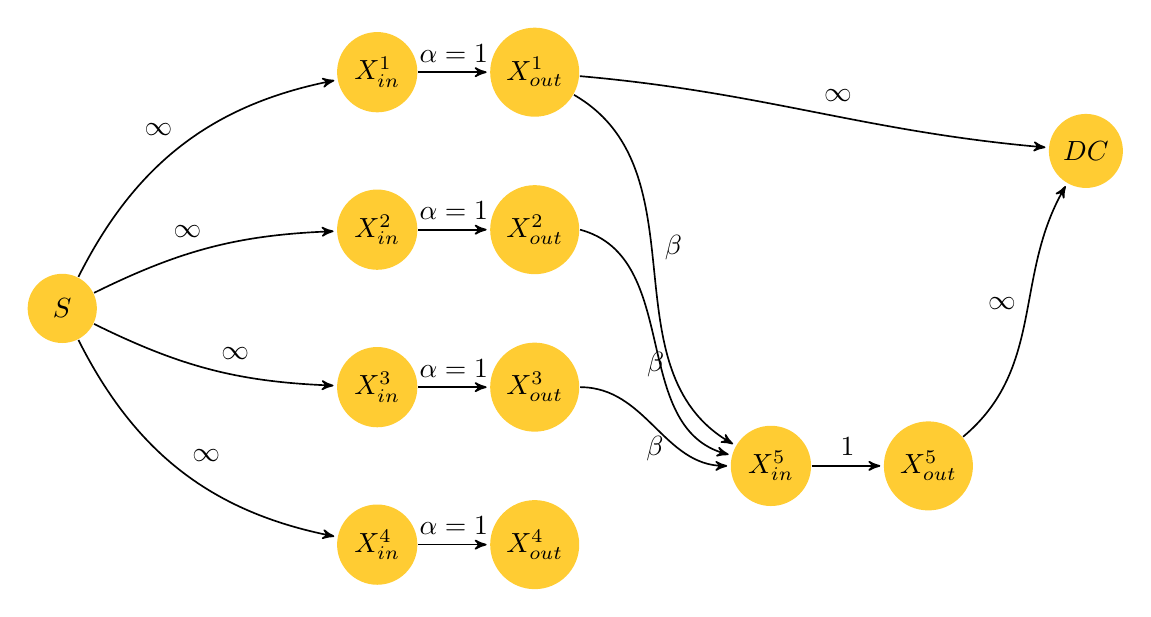
\begin{tikzpicture}[->,>=stealth',shorten >=1pt,auto,node distance=2.8cm,
                    semithick]
  \tikzstyle{every state}=[fill=yellow1,draw=none,text=black]

  \node[state]         (S) at (-6, 0)              {$S$};
  \node[state]         (xin1) at (-2, 3)           {$X^1_{in}$};
  \node[state]         (xin2) at (-2, 1)        {$X^2_{in}$};
  \node[state]         (xin3) at (-2, -1)       {$X^3_{in}$};
  \node[state]         (xin4) at (-2, -3)           {$X^4_{in}$};
  \node[state]         (xout1) at (0, 3)          {$X^1_{out}$};
  \node[state]         (xout2) at (0, 1)        {$X^2_{out}$};
  \node[state]         (xout3) at (0, -1)   {$X^3_{out}$};
  \node[state]         (xout4) at (0, -3)           {$X^4_{out}$};
  \node[state]         (xin5)  at (3, -2)   {$X^5_{in}$};
  \node[state]         (xout5) at (5, -2)   {$X^5_{out}$};
  \node[state]         (DC) at (7, 2)           {$DC$};

  \path (S) edge[bend left=26]              node {$\infty$} (xin1)
            edge[bend left=12]              node {$\infty$} (xin2)
            edge[bend right=12]             node {$\infty$} (xin3)
            edge[bend right=26]             node {$\infty$} (xin4)
        (xin1) edge  node {$\alpha=1$} (xout1)
        (xin2) edge  node {$\alpha=1$} (xout2)
        (xin3) edge  node {$\alpha=1$} (xout3)
        (xin4) edge  node {$\alpha=1$} (xout4)
        (xin5) edge  node {$1$} (xout5);
  \draw[->] (xout1) to[out=-30,in=150] node {$\beta$} (xin5);
  \draw[->] (xout2.east) to[out=-15,in=165] node [below] {$\beta$} (xin5);
  \draw[->] (xout3.east) to[out=0,in=180] node [below] {$\beta$} (xin5.west);
  \draw[->] (xout1) to[out=-5,in=175] node {$\infty$} (DC);
  \draw[->] (xout5) to[out=40, in=-120] node {$\infty$} (DC);
\end{tikzpicture}



\end{flushleft}
\end{document}
